%%%%%%%%%%%%%%%%%%%%%%%%%%%%%%%%%%%%%%%%%%%%%%%%%%%%%%%%%%%%%%%%%%%%%%%%%%%%%%%%%%
\begin{frame}[fragile]\frametitle{}
\begin{center}
{\Large Conclusion}
\end{center}
\end{frame}

%%%%%%%%%%%%%%%%%%%%%%%%%%%%%%%%%%%%%%%%%%%%%%%%%%%%%%%%%%%
\begin{frame}\frametitle{If you have grasped RL by now, then, Test}
As you have come so far, lets see if you can solve the following:

\begin{itemize}
% \item How would you find a minimum of $y=e^(2 - x) + x^2 - x/2$?
% \item Transformers: can you have 5 attention heads with a sequence length equal to 100 and embedding dimension to 512, and why?
\item Please explain why the Bellman Equation is important and explain how you have used it in your work.
\item DQN RL: how can you use DQN on an environment with 100 unique states, and actions taking values on the interval $[-0.5, 0.5]$?
\end{itemize}

{\tiny (Ref: ``Reinforcement Learning Expert'' - MSBAI)}

If, there is a long way to go \ldots  Next are some of the learning resources \ldots
\end{frame}



%%%%%%%%%%%%%%%%%%%%%%%%%%%%%%%%%%%%%%%%%%%%%%%%%%%%%%%%%%%
\begin{frame}[fragile]\frametitle{Learning Resources}
\begin{center}
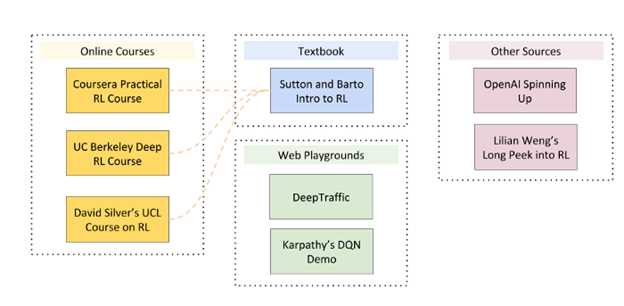
\includegraphics[width=\linewidth,keepaspectratio]{rl24}
\end{center}
{\tiny (Ref: Newbie’s Guide to Study Reinforcement Learning - Towards Data Science)}
\end{frame}

%%%%%%%%%%%%%%%%%%%%%%%%%%%%%%%%%%%%%%%%%%%%%%%%%%%%%%%%%%%
\begin{frame}\frametitle{RL for AI Safety}

\begin{itemize}
\item Deep reinforcement learning to play role in AI Safety
\item To prepare: not yet a standard deep RL textbook, most of the knowledge is locked up in either papers; takes a long time to digest.
\item Deep RL algorithms are painful due to obscure papers and public implementations.
\item Open AI Spinning Up is a useful Library.
\item Has algorithms like DDPG and Q-Learning are off-policy, so they are able to reuse old data very efficiently. 
\item Has Vanilla Policy Gradient, a on-policy algorithm: that is, they don’t use old data, which makes them weaker on sample efficiency. 
\end{itemize}

{\tiny (Ref: ``Spinning Up'' - OpenAI)}

\end{frame}
